\section{Results}
\label{sec:Results}
In this section, we evaluate the effectiveness of our approach, and compare its performance with state-of-the-art methods including N-ICP~\cite{amberg2007optimal}, RPTS~\cite{li2018robust}, and SVR-$\ell_0$~\cite{guo2015robust}. The evaluations are performed on the MPI Faust dataset~\cite{Bogo:CVPR:2014} and the human motion datasets from~\cite{vlasic2008articulated}. We only show representative results in this section, with more comparisons provided in the supplementary material.


\begin{figure}[!t]
	\centering
	 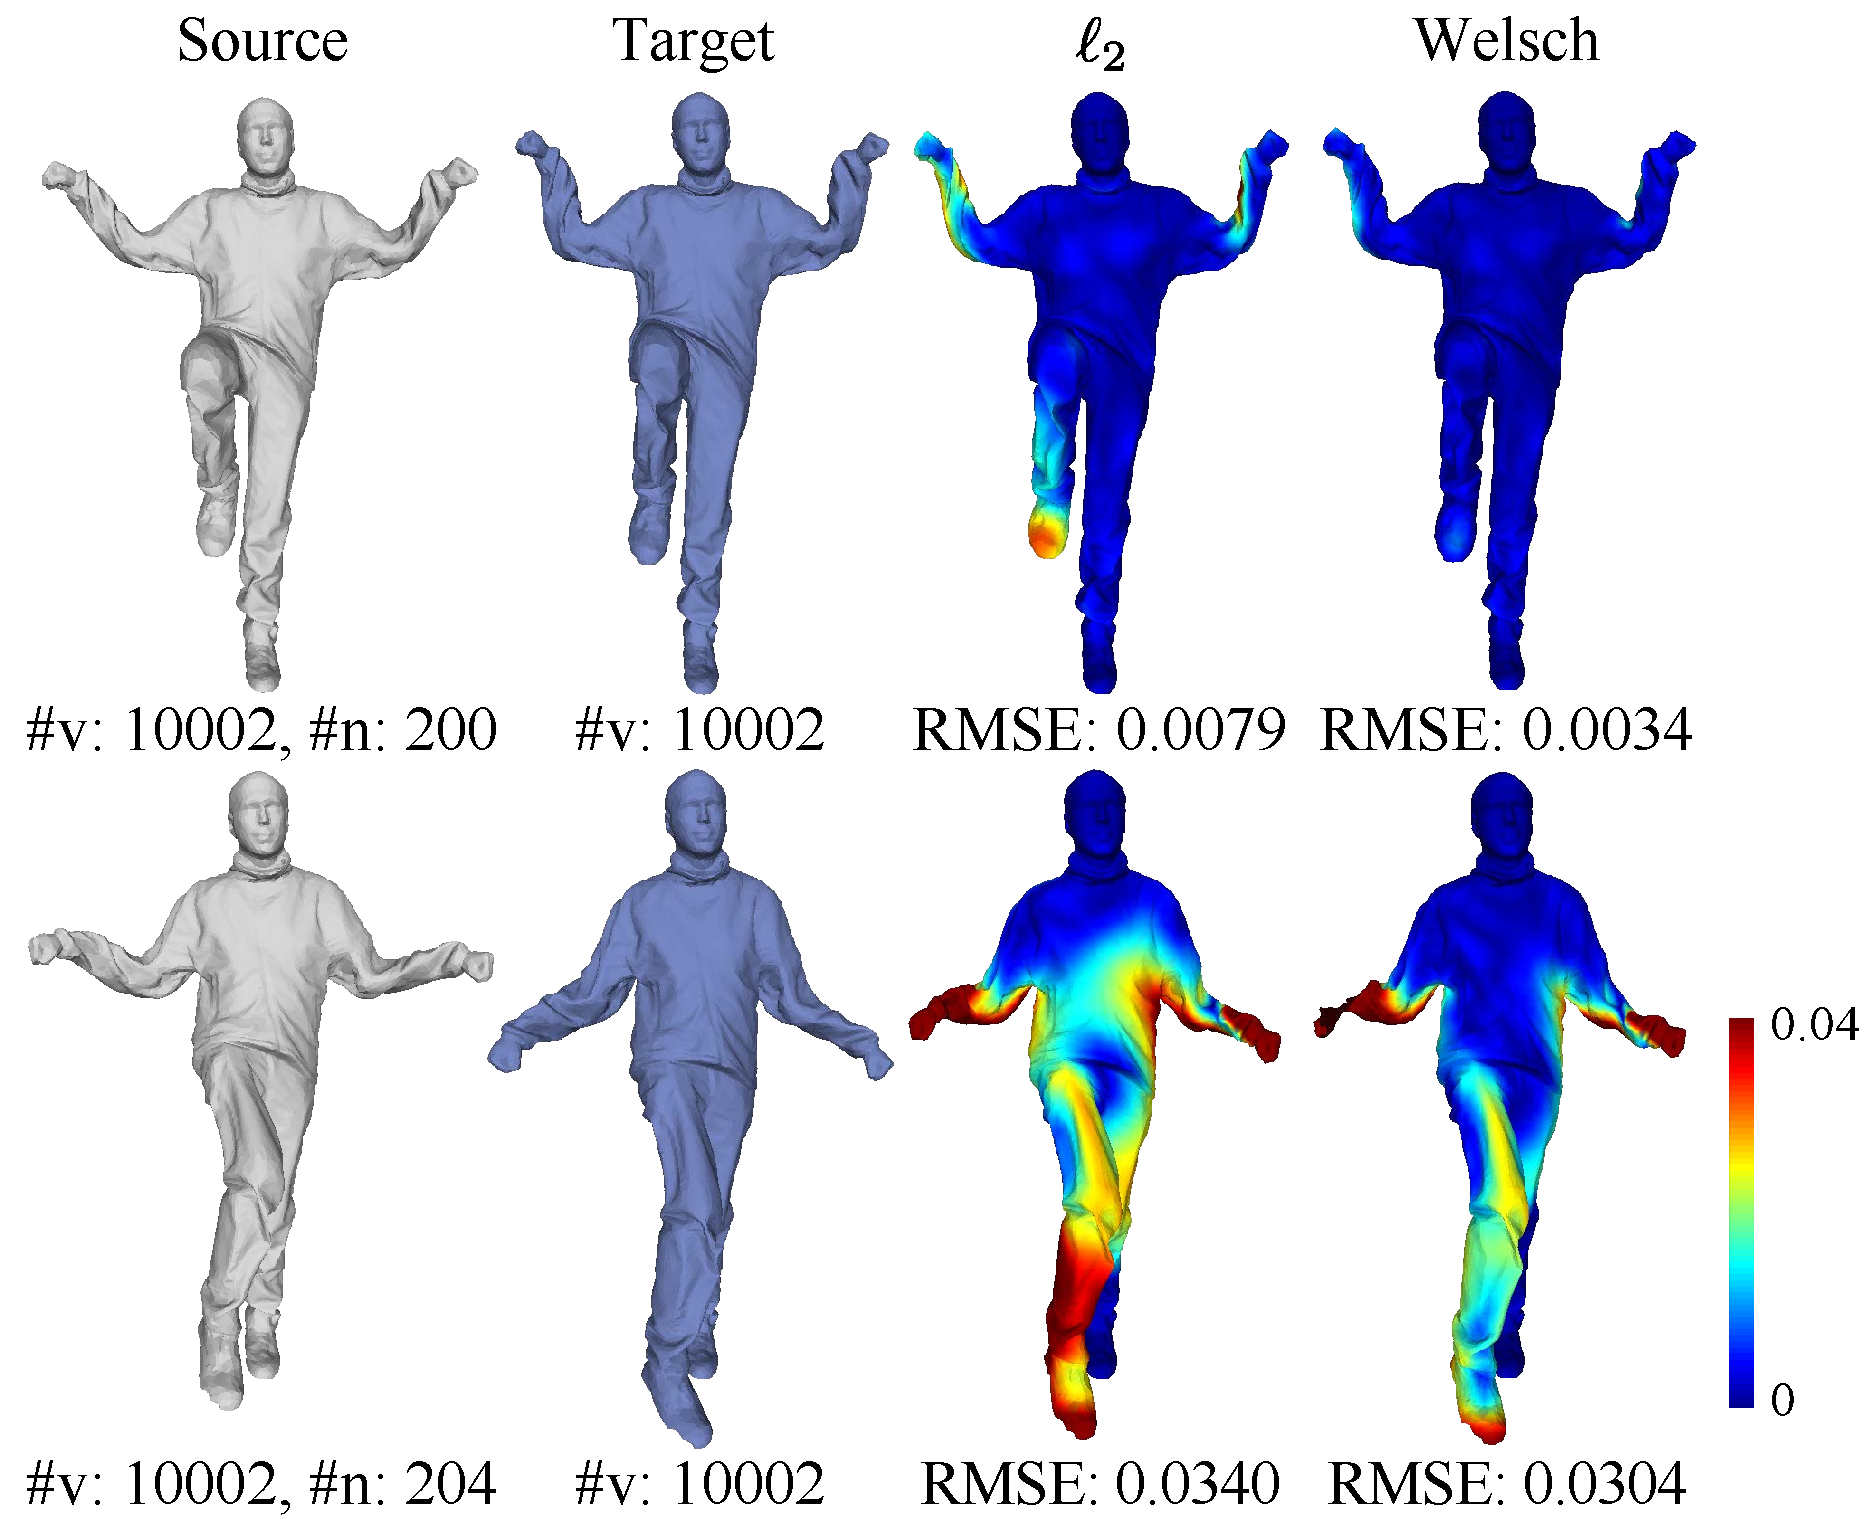
\includegraphics[width=\columnwidth]{Figs/comparel2.pdf}
	\caption{Comparison between our formulation and an alternative formulation using the $\ell_2$-norm instead of the Welsch's function, tested on two pairs of meshes from the ``crane'' dataset of~\cite{vlasic2008articulated}. We set with $k_{\alpha} = 0.1, k_{\beta} = 100$ for the $\ell_2$-norm formulation, and $k_{\alpha} = 1, k_{\beta} = 10^4$ for our formulation.}
\vspace{-5mm}
	\label{fig:compare_l2}
\end{figure}

\paragraph{Implementation Details}
We implement our method in C++, and all results and comparisons are tested on a PC with 16GB of RAM and a 6-core CPU at 3.60GHz.
Each pair of surfaces are pre-processed by aligning their centroids and scaling them to achieve unit-length diagonal for their combined bounding box.
We initialize the transformation variables using a rigid transformation computed via 15 iterations of the ICP algorithm to align the source and target points, with rejection of point pairs whose distance is larger than a threshold $\epsilon_d$ or whose normal vectors deviate by more than an angle $\theta$~\cite{Rusinkiewicz2001}. We set $\epsilon_d = 0.3$ and $\theta = 60^\circ$ by default. The ICP iterations are initialized by aligning corresponding feature points, determined either using the closest point pairs between the pre-processed surfaces coupled with the above rejection criteria, or using the SHOT feature~\cite{tombari2010unique} with diffusion pruning~\cite{tam2014diffusion}, or through manual labeling.
In the figures, we visualize the initial correspondence using blue lines connecting the corresponding points.
We evaluate the registration accuracy via the root mean square error compared with the ground truth:
\begin{equation}
\text{RMSE}=\sqrt{\frac{\sum_{\mathbf{v}_i \in{\mathcal{V}}}e_i^2}{|\mathcal{V}|}},
\end{equation}
where $e_i  = \|\mathbf{v}_i^{\ast} -\mathbf{v}_i^{\text{gt}}\|$
is the deviation between the transformed positions $\mathbf{v}_i^{\ast}, \mathbf{v}_i^{\text{gt}}$ of a source point $\mathbf{v}_i$ under the computed and the ground-truth transformations respectively. In the figures, we show the RMSE for each registration result, and use color-coding to visualize the error values $\{e_i\}$ across the surface. Unless stated otherwise, all RMSE values and color-coded registration errors are in the unit of meters. We use $\#$v to denote the number of sample points on a surface, and $\#$n for the number of deformation graph vertices.
Similar to our formulation~\eqref{eq:model}, the optimization target functions of N-ICP, RPTS, and SVR-$\ell_0$ all involve a regularization term and/or a term for the rigidity of transformations. To ease presentation, for all methods we use $\alpha$ and $\beta$ to denote the weights for the regularization term and the rigidity term, respectively. We tune the weights for each method to obtain their best results for comparison.
In addition, N-ICP and RPTS require dropping unreliable correspondence between source and target points in each iteration, and we adopt the distance and normal deviation thresholds $\epsilon_d$ and $\theta$ as used in the ICP iterations for initialization.



\begin{figure}[!t]
	\centering
	 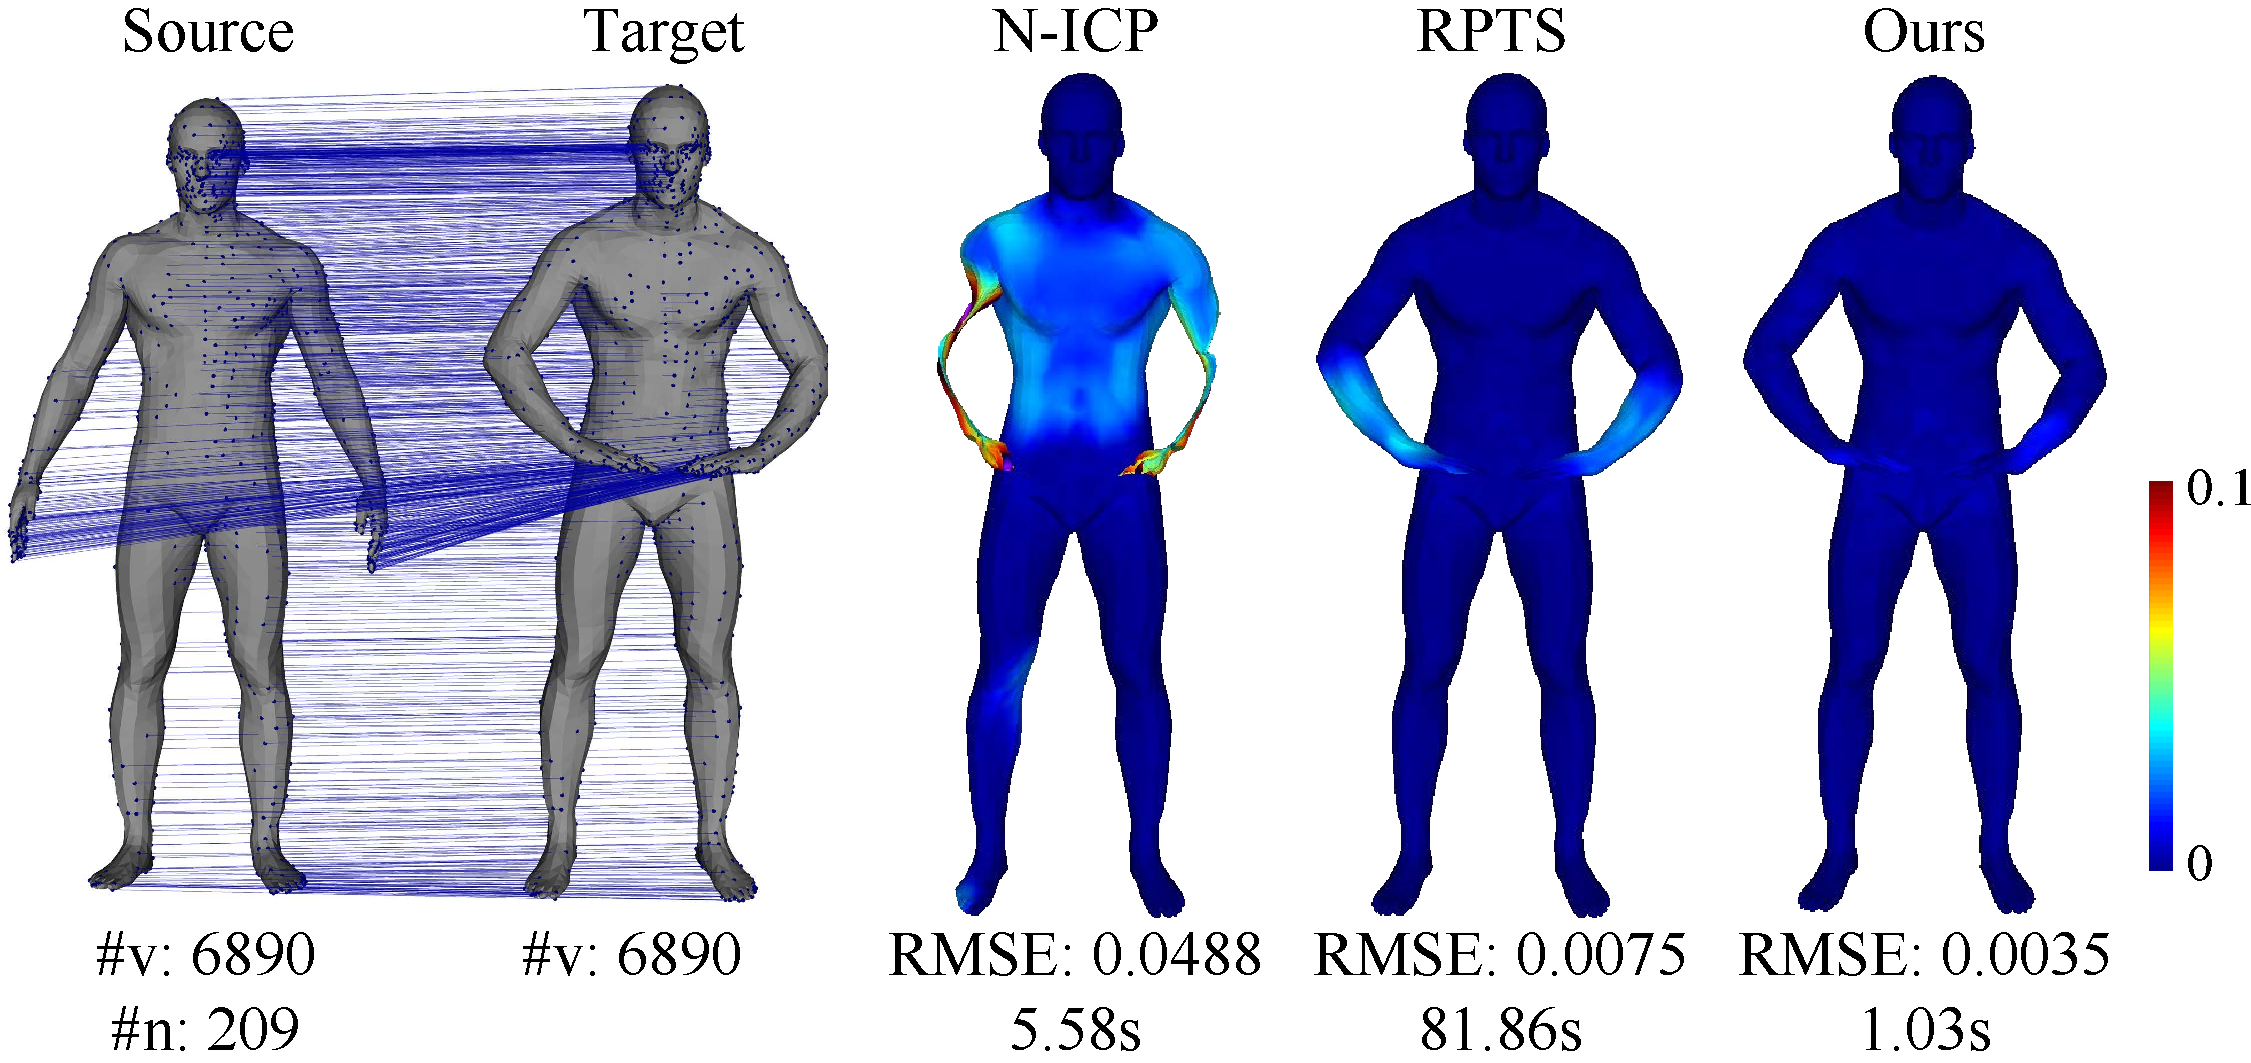
\includegraphics[width=\columnwidth]{Figs/clean.pdf}   \caption{Comparison of registration results on an example from the MPI Faust dataset.}
	\label{fig:faust}
\end{figure}

\begin{table}[!t]
	\caption{Average computation time and RMSE (in millimeters) on the MPI Faust dataset. We set $\alpha = 5$ for N-ICP,  $\alpha = 100, \beta = 0.1$ for RPTS, and $k_{\alpha} = k_{\beta} = 0.001$ for our method.}
	\label{Tab:faust}
	\setlength{\tabcolsep}{1.6pt}
	\centering
	\begin{small}
		\begin{tabular}{ | c |  c  c | c  c | c  c | c  c  |}
			\Xhline{1pt}
			\multicolumn{1}{ | c |}{\multirow{2}{*}{Pose Pair}}
			&\multicolumn{2}{ c |}{N-ICP}
			&\multicolumn{2}{ c | }{RPTS}
			&\multicolumn{2}{ c |}{Ours}    \\\cline{2-7}
			%\midrule
			\multicolumn{1}{ | c |}{}
			&Time  (s)     &RMSE
			&Time  (s)     &RMSE
			&Time  (s)     &RMSE \\\hline
	        1 & 7.43  & 59.7  & 61.83  & 9.16  & \textbf{1.24}  & \textbf{5.46} \\
        2 & 4.46  & 20.8  & 46.52  & 3.22  & \textbf{0.86}  & \textbf{1.35} \\
        3 & 7.95  & 80.1  & 35.25  & \textbf{7.97}  & \textbf{1.36}  & 8.99 \\
        4 & 5.45  & 45.4  & 22.99  & 5.69  & \textbf{1.27}  & \textbf{4.26} \\
        5 & 4.13  & 14.2  & 14.04  & \textbf{0.717}  & \textbf{0.81}  & 1.06 \\
        6 & 8.61  & 59.6  & 28.72  & 6.29  & \textbf{1.30}  & \textbf{3.89} \\
        7 & 12.57  & 208  & 43.26  & 61.6  & \textbf{2.23}  & \textbf{49.3} \\
        8 & 6.05  & 70.4  & 26.27  & \textbf{6.58}  & \textbf{1.34}  & 7.54 \\\hline
        Mean & 7.08  & 69.7  & 34.86  & 12.7  & \textbf{1.30}  & \textbf{10.2} \\
        Median & 6.74  & 59.6  & 31.99  & 6.44  & \textbf{1.28}  & \textbf{4.86} \\
			\Xhline{1pt}
		\end{tabular}
	\end{small}
\end{table}



\subsection{Effectiveness of the Welsch's Function}
We perform the optimization~\eqref{eq:model} with the Welsch's functions in $E_{\text{align}}$ and $E_{\text{reg}}$ replaced by square functions. Fig.~\ref{fig:compare_l2} compares the registration accuracy of such $\ell_2$-norm formulation with our approach, on two problem instances from the ``crane'' dataset of~\cite{vlasic2008articulated}. we can see that the Welsch's function leads to more accurate results than the $\ell_2$-norm.


\begin{figure}[!t]
	\centering
	 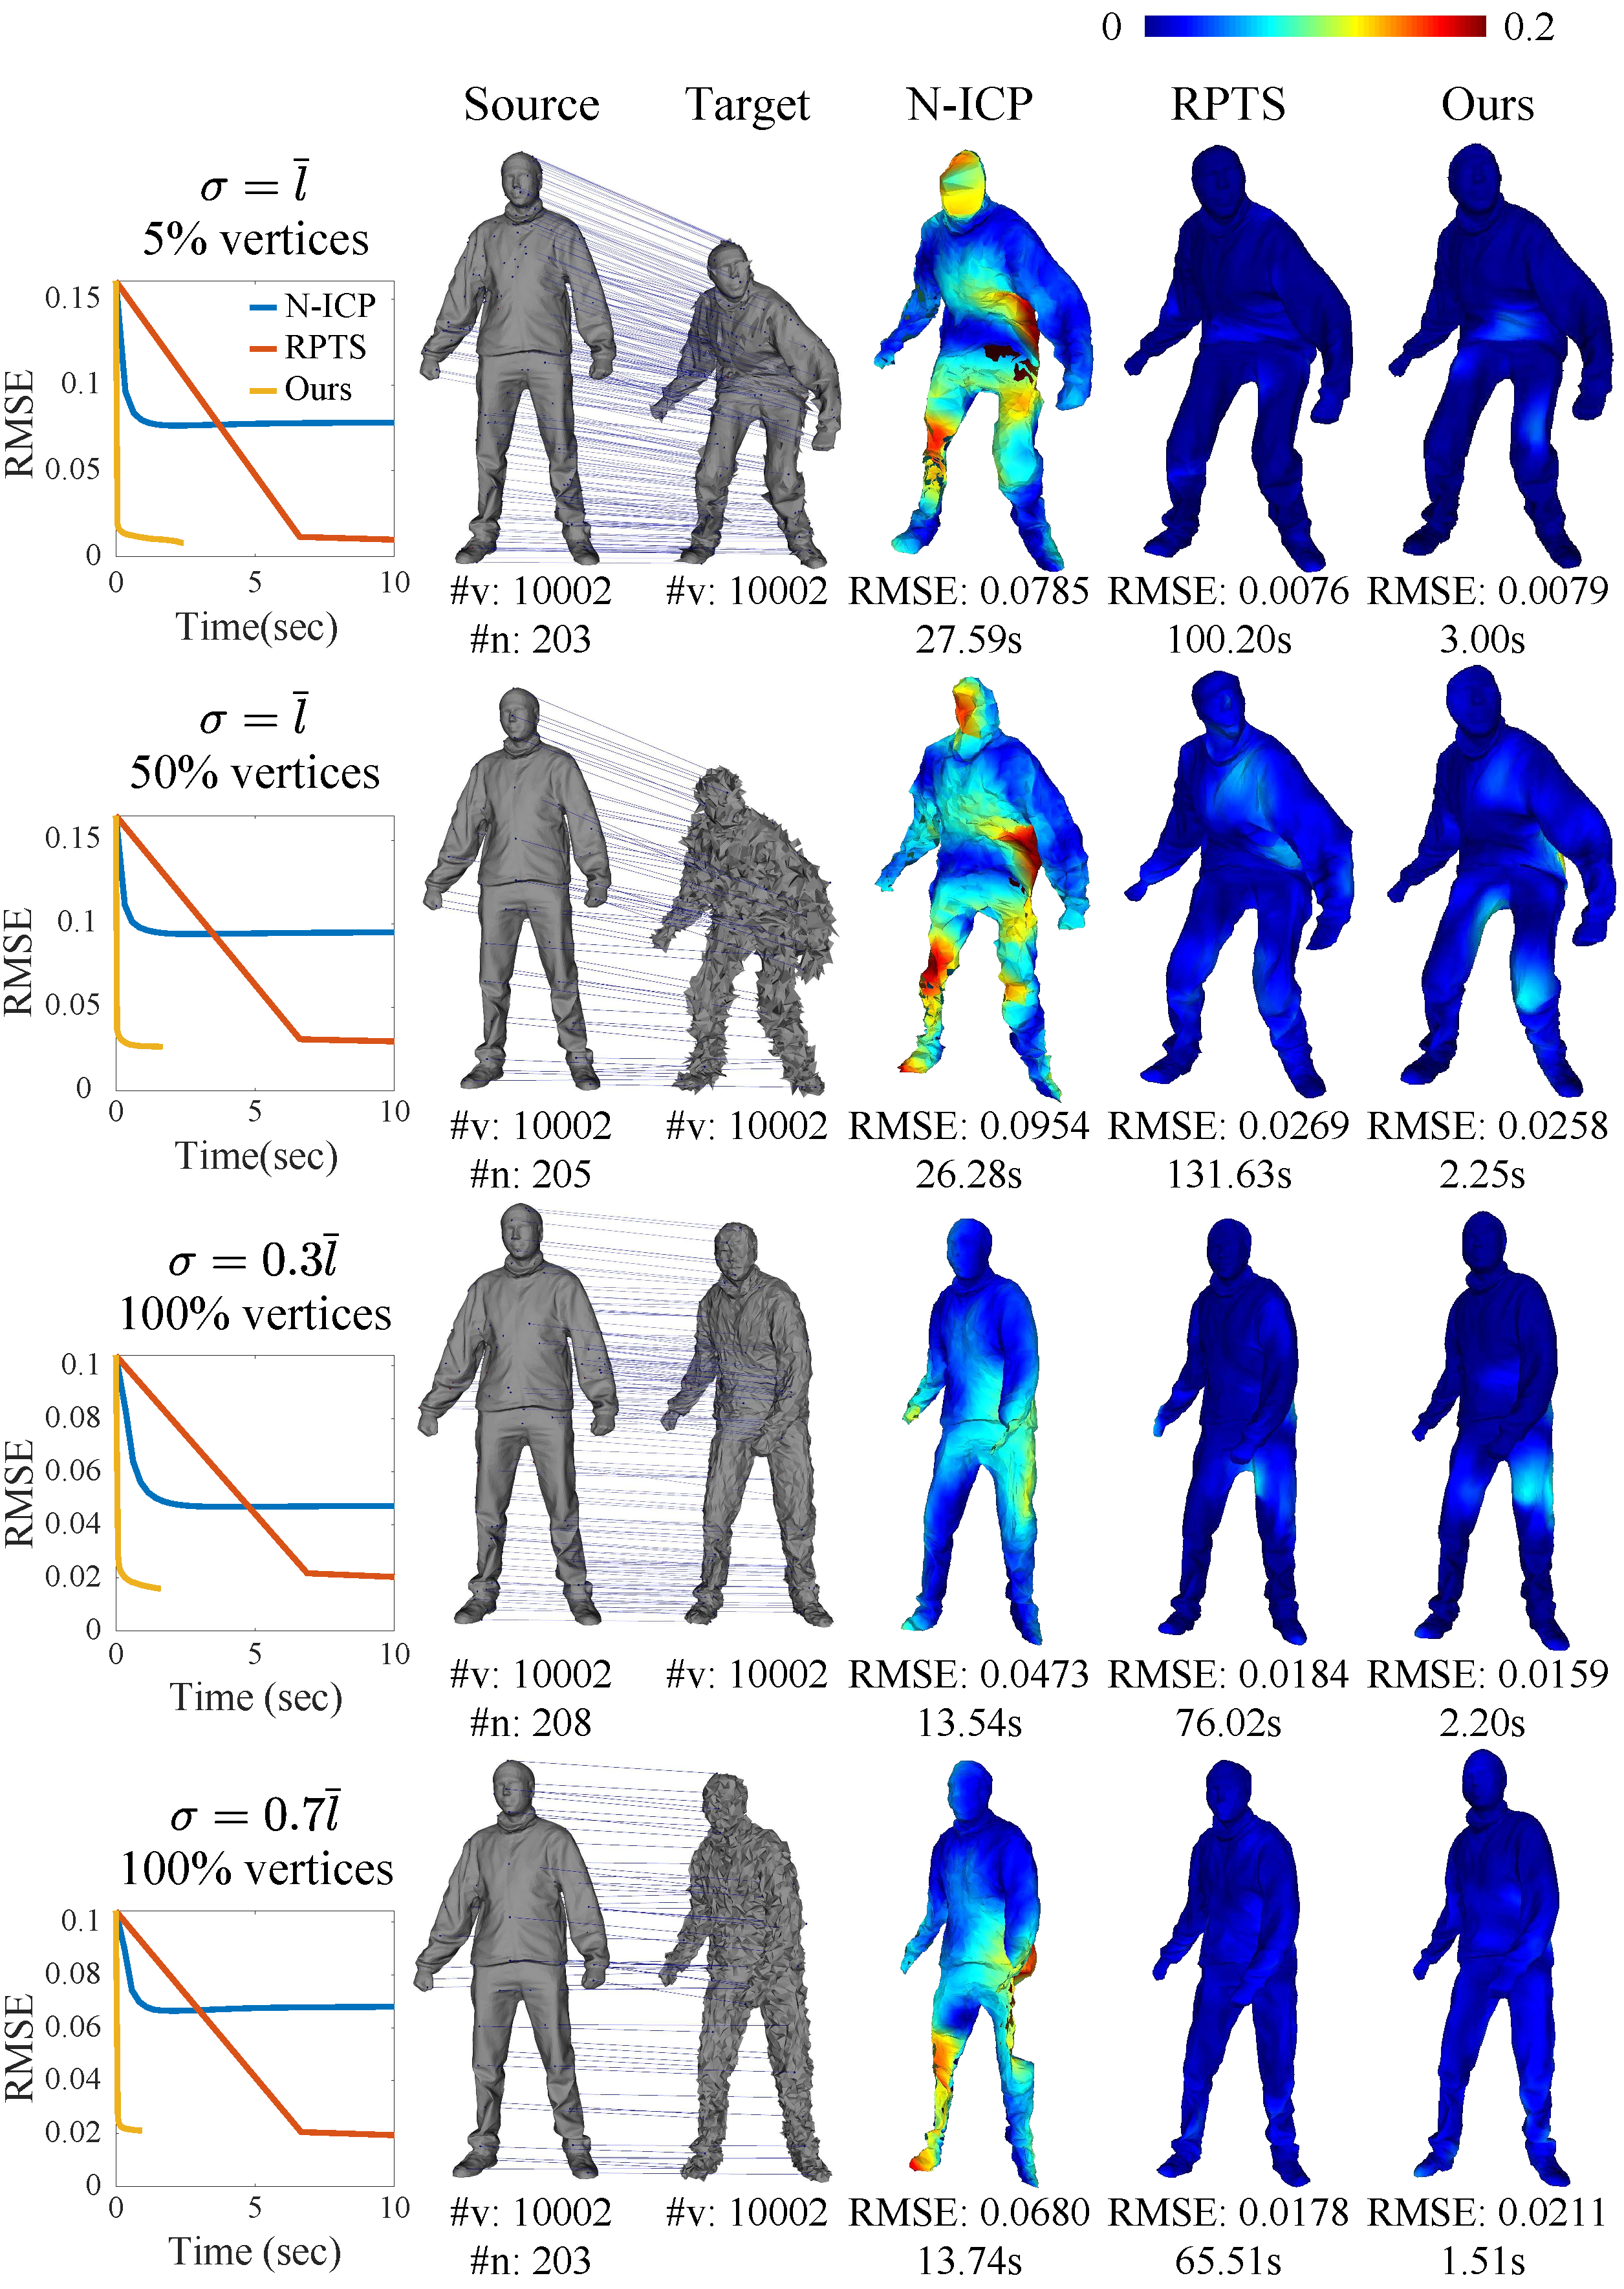
\includegraphics[width=\columnwidth]{Figs/noise.pdf}
	\caption{Comparison with N-ICP and RPTS on noisy models constructed by adding Gaussian noise to some vertices on the target surface. The original models are taken from the ``jumping'' dataset of~\cite{vlasic2008articulated}. The left column shows how the RMSE of registration results changes over time during optimization. We set $\alpha = 5$ for N-ICP, $\alpha = 10, \beta = 1$ for RPTS, $k_{\alpha} = 0.01, k_{\beta} = 1$ for our method, and $\theta=180^\circ$ for all methods.}
\vspace{-5mm}
	\label{fig:noise}
\end{figure}



\subsection{Comparison with Other Methods}
In Tab.~\ref{Tab:faust} and Fig.~\ref{fig:faust}, we compare our method with N-ICP and RPTS on the MPI Faust dataset.
We select 10 subjects with 9 poses, and use the first pose of each subject as the source surface the other poses of the subject as the targets.
We evaluate the average RMSE among all subjects for the same pose pair, and list them in Tab.~\ref{Tab:faust}.
Fig.~\ref{fig:faust} shows the results from different methods on a pose pair for a subject. We can see that our method requires significantly less computational time while achieving similar or better accuracy. A major reason for the efficiency of our method is the adoption of a deformation graph, which only requires optimizing one affine transformation per graph vertex. In comparison, N-ICP and RPTS require optimizing one affine transformation per mesh vertex, which significantly increases the number of variables as well as computational time.








Fig.~\ref{fig:noise} compares our method with N-ICP and RPTS on models from the ``jumping'' dataset of~\cite{vlasic2008articulated}, with added Gaussian noise on vertex positions of the target surface along their normal directions.
In the first two rows of Fig.~\ref{fig:noise}, we add noise with standard deviation $\sigma = \overline{l}$ to 5\% or 50\% of the vertices on the target surface respectively, where $\overline{l}$ is the average edge length of the target surface.
In the last two rows, we add noise to all vertices of the target surface with stand deviation $\sigma = 0.3 \overline{l}$ and $\sigma = 0.7 \overline{l}$, respectively.
The comparison shows that our method is more robust to noisy data.

In Fig.~\ref{fig:partial}, we compare our method with  N-ICP, RPTS and SVR-$\ell_0$ on partially overlapping data, which is synthesized from the ``bouncing'' dataset of~\cite{vlasic2008articulated} by removing some vertices from the target surface. For SVR-$\ell_0$, we use the squared distance from source points to their closest target points as the data fitting term. We can see that our method is significantly faster than other methods, and is more robust to such partial overlapping model.

\begin{figure}[!t]
	\centering
	 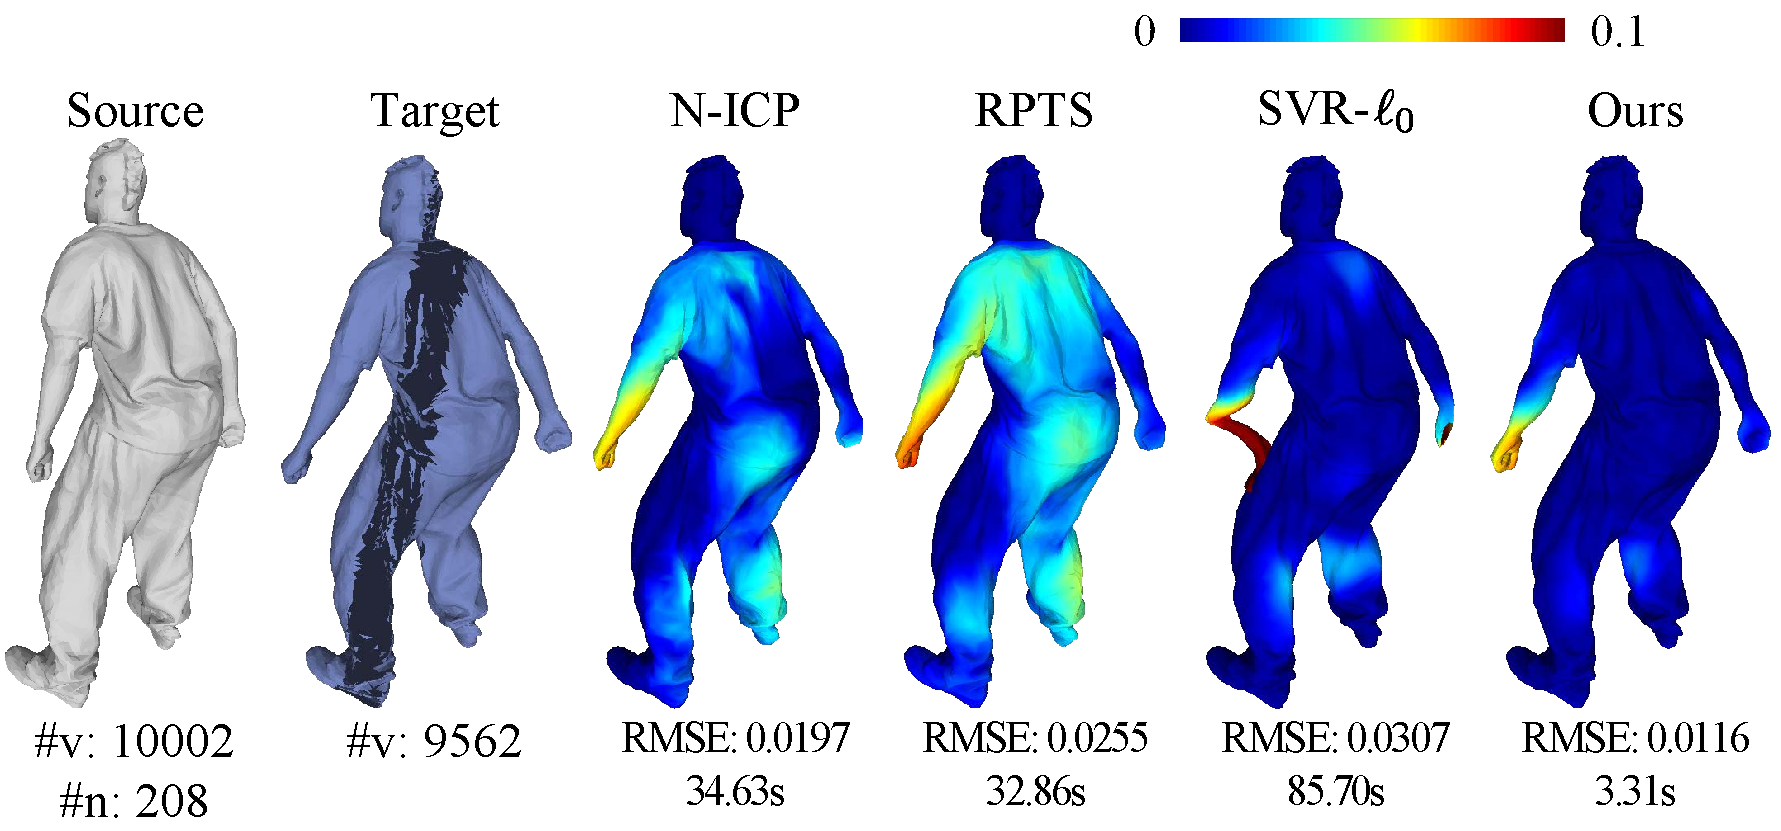
\includegraphics[width=1\columnwidth]{Figs/partial.pdf}
	\caption{Comparison with N-ICP, RPTS and SVR-$\ell_0$ on models with partial overlaps, constructed by removing some vertices from the target surface. The original models are taken from the ``bouncing'' dataset of~\cite{vlasic2008articulated}. We set $\alpha = 10$ for N-ICPS, $\alpha = 1, \beta=100$ for RPTS, $\alpha = 0.1,\beta = 100$ for SVR-$\ell_0$, $k_{\alpha} = 1, k_{\beta} = 100, \nua^{\max}=30\overline{d}, \nur^{\max} = 100\overline{l}$ for our method, and $ \theta=45^\circ$ for all methods.}
\vspace{-5mm}
	\label{fig:partial}
\end{figure}
